\documentclass{article}

% if you need to pass options to natbib, use, e.g.:
% \PassOptionsToPackage{numbers, compress}{natbib}
% before loading nips_2016
%
% to avoid loading the natbib package, add option nonatbib:
% \usepackage[nonatbib]{nips_2016}

%\usepackage{nips_2016}

% to compile a camera-ready version, add the [final] option, e.g.:
 \usepackage[final]{nips_2016}

\usepackage[utf8]{inputenc} % allow utf-8 input
\usepackage[T1]{fontenc}    % use 8-bit T1 fonts
\usepackage{hyperref}       % hyperlinks
\usepackage{url}            % simple URL typesetting
\usepackage{booktabs}       % professional-quality tables
\usepackage{amsfonts}       % blackboard math symbols
\usepackage{nicefrac}       % compact symbols for 1/2, etc.
\usepackage{microtype}      % microtypography
\usepackage{tikz}
\usetikzlibrary{fit,positioning}
\usepackage{amsmath}
\usepackage[round]{natbib}

\title{Varying Variational Autoencoders}

% The \author macro works with any number of authors. There are two
% commands used to separate the names and addresses of multiple
% authors: \And and \AND.
%
% Using \And between authors leaves it to LaTeX to determine where to
% break the lines. Using \AND forces a line break at that point. So,
% if LaTeX puts 3 of 4 authors names on the first line, and the last
% on the second line, try using \AND instead of \And before the third
% author name.

\author{
  Nathan Kong \\
  University of Toronto\\
  \texttt{nathan.kong@mail.utoronto.ca} \\
  %% examples of more authors
  \And
  Jingyao (Jason) Li \\
  University of Toronto \\
  \texttt{jasons\_email@toronto.edu}\\
  %% Address \\
  %% \texttt{email} \\
  %% \AND
  %% Coauthor \\
  %% Affiliation \\
  %% Address \\
  %% \texttt{email} \\
  %% \And
  %% Coauthor \\
  %% Affiliation \\
  %% Address \\
  %% \texttt{email} \\
  %% \And
  %% Coauthor \\
  %% Affiliation \\
  %% Address \\
  %% \texttt{email} \\
}

\newcommand{\E}{\mathbb{E}}
\newcommand{\bz}{\mathbf{z}}
\newcommand{\bx}{\mathbf{x}}
\newcommand{\given}{\,|\,}
\newcommand{\D[1]}{\mathrm{d}{#1}}
\newcommand{\KL}{\mathbb{D}_{\text{KL}}}

\begin{document}

\maketitle

\begin{abstract}
In variational inference, the approximate posterior distribution that is chosen is very important.  It
needs to be computationally tractable, yet flexible enough to approximate the true posterior.  In this 
paper, we discuss an application of variational inference in dimensionality reduction.  We experiment
with the variational autoencoder (VAE), which was developed by \citet{KW13}, by comparing two
different variational inference methods.  The first method is the vanilla VAE and the second method
improves variational inference by introducing normalizing flows, developed by \citet{RM15}, which 
increases the complexity of an initial simple distribution, so that more complex true posteriors can
be potentially approximated.
\end{abstract}

\section{Introduction}
Nowadays, with increasingly large amounts of data, making posterior inferences is intractable 
since the evidence in Bayes' Rule consists of a computationally intractable integral.  Stochastic 
variational inference was developed that makes this inference more tractable, by turning the 
inference problem into an optimization problem.


\section{Formal Description}

\begin{figure}[htdp]
\centering
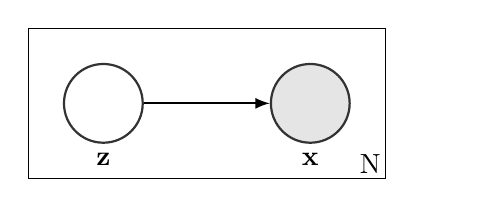
\begin{tikzpicture}
\tikzstyle{main}=[circle, minimum size = 10mm, thick, draw =black!80, node distance = 16mm]
\tikzstyle{connect}=[-latex, thick]
\tikzstyle{box}=[rectangle, draw=black!100]
  \node[main] (z) [label=below:$\bz$] {};
  \node[main, fill = black!10] (x) [right=of z,label=below:$\bx$] { };
  \path (z) edge [connect] (x);
  \node[rectangle, inner sep=0mm, fit= (z) (x),label=below right:N, xshift=13mm] {};
  \node[rectangle, inner sep=4.4mm,draw=black!100, fit= (z) (x)] {};
\end{tikzpicture}
\caption{Probabilistic graphical model with latent variables, $\bz$, and observed variables, $\bx$.}
\label{fig:problem_pgm}
\end{figure}

From a probabilistic graphical model perspective, we have a latent space, governed by $\bz$,
and an observed space, which are our data, $\bx$.  The observed variables depend on the
latent variables.  Figure \ref{fig:problem_pgm} illustrates this model.  Using this framework,
the joint density is: $p(\bx,\bz) = p(\bx \given \bz)\,p(\bz)$. $p(\bz)$ is the prior over the latent 
variables and $p(\bx \given \bz)$ is the likelihood of the data given the latent variables.

\subsection{Variational Lower Bound}
In order to obtain the marginal likelihood $p(\bx)$, we must integrate over $\bz$, which is intractable.  
So, a posterior distribution, $q(\bz \given \bx)$, is introduced allowing us to obtain a lower bound on 
the marginal likelihood:
\begin{align}
	\log p(\bx) &= \log\int_{\bz} p(\bx \given \bz)\,p(\bz)\,\D[\bz] \\
			&= \log\int_{\bz} \frac{q(\bz \given \bx)}{q(\bz \given \bx)}p(\bx \given \bz)\,p(\bz)\,\D[\bz] \label{eq:evid} \\
			&\geq \E_q\left[\log p(\bx,\bz)\right] - \E_q\left[\log q(\bz \given \bx)\right] \label{eq:pq_lb} \\
			&= \log p(\bx) - \KL\left[q(\bz \given \bx) \,||\, p(\bz \given \bx)\right] \label{eq:KL_evid} \\
			&= -\KL\left[q(\bz \given \bx) \,||\, p(\bz)\right] + \E_{q(\bz \given \bx)}\left[\log p(\bx \given \bz)\right] \label{eq:ELBO}
\end{align}

Equation \ref{eq:pq_lb} follows from Equation \ref{eq:evid} by applying Jensen's inequality.  Equation 
\ref{eq:ELBO} is known as the variational lower bound, which we want to maximize.  Note that from
Equation \ref{eq:KL_evid}, maximizing the lower bound minimizes the Kullback-Leibler (KL) divergence 
between the approximate posterior and the true posterior and maximizes the marginal likelihood since
the KL divergence is always positive.  We want $q(\bz \given \bx)$ to be computationally tractable, but
flexible enough to be able to match $p(\bz \given \bx)$ such that the KL divergence is close to 0.

\subsection{Vanilla VAE}

In an autoencoder, there are two main stages: the encoder stage and the decoder stage, which are
both neural networks.  The input to the encoder, or recognition, stage is the high dimension feature 
vector that we want to reduce to a space with lower dimensionality.  In a VAE, the output of the 
encoder stage are parameters to the approximate posterior, $q(\bz \given \bx)$.  If $q(\bz \given \bx)$
is a Gaussian, the parameters would be the mean, $\boldsymbol{\mu}$, and variance, $\boldsymbol{\sigma}^2$.
In this case, the covariance matrix is a diagonal matrix.

We want to minimize the negative ELBO (negative of Equation \ref{eq:ELBO}) to train the VAE.  It is: 
$\KL\left[q(\bz \given \bx) \,||\, p(\bz)\right] - \E_{q(\bz \given \bx)}\left[\log p(\bx \given \bz)\right]$
The first term measures how different the approximate posterior is from $p(\bz)$, so that a smaller value
indicates a better approximation.  The second term is the reconstruction error.

\subsection{VAE with Normalizing Flow}

\section{Related Work}



\section{Comparison}

\subsection{Baseline VAE}
For the vanilla VAE, we want to maximize the variational lower bound or minimize the negative variational
lower bound.


\subsection{VAE with Normalizing Flow}
In \citet{RM15}, variational inference is improved by introducing normalizing flows.  Recall that in
variational inference, we want $q(\bz \given \bx)$ to be flexible enough to approximate the true posterior,
$p(\bz \given \bx)$, since the true posterior can be extremely complicated.


\section{Limitations}

\section{Conclusions}


\small
%\bibliographystyle{IEEEtranN}
\bibliographystyle{plainnat}
\bibliography{references.bib}


\end{document}